\section{Розробка та тестування програмного забезпечення}
\subsection{Планування тестування програмного забезпечення}
\subsubsection{Загальна теорія тестування}
Тестування --- перевірка відповідності реальної поведінки програми очікуваній, що здійснюється на кінцевому наборі тестів, який був обраний певним чином. 
У більш широкому сенсі, тестування --- це одна з технік контролю якості, що включає в себе активності з планування робіт, проектування тестів, виконання тестування і аналізу отриманих результатів.

Верифікація --- це процес оцінки системи або її компонентів з метою визначення чи задовольняють результати поточного етапу розробки умовам, що були сформовані на початку цього етапу. 
Тобто чи виконуються наші цілі, терміни, завдання по розробці проекту, визначені на початку поточної фази.

Валідація --- це визначення відповідності ПО, що розроблюється очікуванням і потребам користувача, вимогам до системи. 

\subsubsection{Порядок проведення тестування програмного забезпечення, що розроблюється}
На першому етапі тестування необхідно провести модульне тестування усіх компонентів системи, які можуть бути протестовані окремо від інших у штучному середовищі тестування. 
Unit-тестування буде проведено за допомогою засобу автоматизації тестування Junit.

Такий вибір зумовлений простотою інтеграції Junit з Kotlin. 
Junit надає великий об'єм валідаційних методів, завдяки яким можна легко та ефективно тестувати як модулі обробки даних та взаємодії з базами даних, так і модулі вводу та виводу інформації.

У подальшому необхідно виконати інтеграційне тестування, що передбачає тестування у двох напрямках.
Інтеграційне тестування компонентного рівня після unit-тестування необхідне для перевірки правильної взаємодії частин бізнес-логіки додатку. 
Завдяки такому тестуванню можна виявити помилки реалізації зовнішніх інтерфейсів або ж їх некоректне використання.

Інтеграційне тестування системного рівня необхідне для знаходження можливих помилок у взаємодії різних підсистем програмного забезпечення, його взаємодії з операційною системою, іншими додатками.
На етапі системного тестування необхідно визначити, чи відповідає розроблена програмне забезпечення визначеним функціональним та нефункціональним вимогам.
Для цього необхідно виконати усі визначені сценарії використання в умовах, що близькі до реальних. 
Даний етап є дуже важливим, тому що існує ризик виявлення таких дефектів, як відсутність або неправильна реалізація функціональності, невиконання таких функціональних вимог, як зручність використання, захищеність, продуктивність тощо. 
На етапі системного тестування виконують остаточну перевірку сумісності програмного забезпечення та операційної системи.

Найвищим рівнем тестування є прийомне тестування, що виконується до тих пір, поки його результати не задовольнять замовника та інших зацікавлених осіб.

\subsection{Графічний інтерфейс програмного забезпечення}
На рисунку~\ref{fig:screenshot} зображено графічний інтерфейс прототипу програмного засобу для моделювання розподільчих логістичних систем.

\begin{figure}[H]
	\centering
	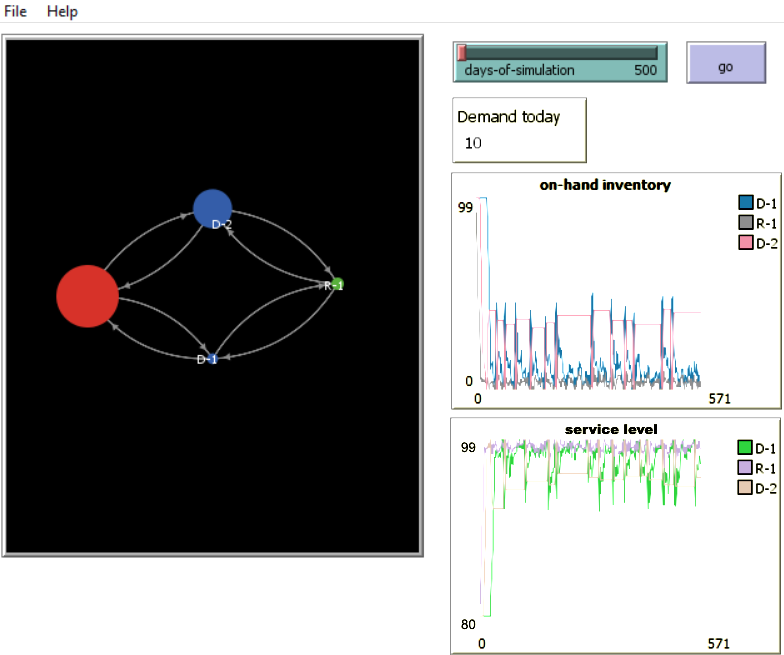
\includegraphics[width=\textwidth]{screenshot}
	\caption{Графічний інтерфейс програмного забезпечення}
	\label{fig:screenshot}
\end{figure} 

Графічний інтерфейс складається з двох частин: меню та панелі поточного стану моделі.

Меню складається з двох пунктів:
\begin{enumerate}[label={\arabic*)}]
	\item File --- пункт, з якого можна загрузити конфігурацію логістичної системи та зробити звіт;
	\item Help --- пункт, в якому міститься базова інформація о програмі та автору.
\end{enumerate} 

Панель поточного стану моделі складається з візуального представлення моделі (де \textit{D-1}, \textit{D-2} --- постачальники, \textit{R-1} --- роздрібний продавець, інше --- головний склад), кнопки запуску симуляції та графіків рівня запасу та рівня сервісу.
